\section{User manual}
Figure~\ref{fig:router} depicts the router configuration. Three components are required to use the board as a DHCP (\textbf{D}ynamic \textbf{H}ost \textbf{C}onfiguration \textbf{P}rotocol) relay:
\begin{itemize}
	\item DHCP server, assigns IP addresses to clients;
	\item DHCP client, requests an IP address;
	\item DHCP relay, bridges between the client and the server.
\end{itemize}

\begin{figure}[h]
	\centering
	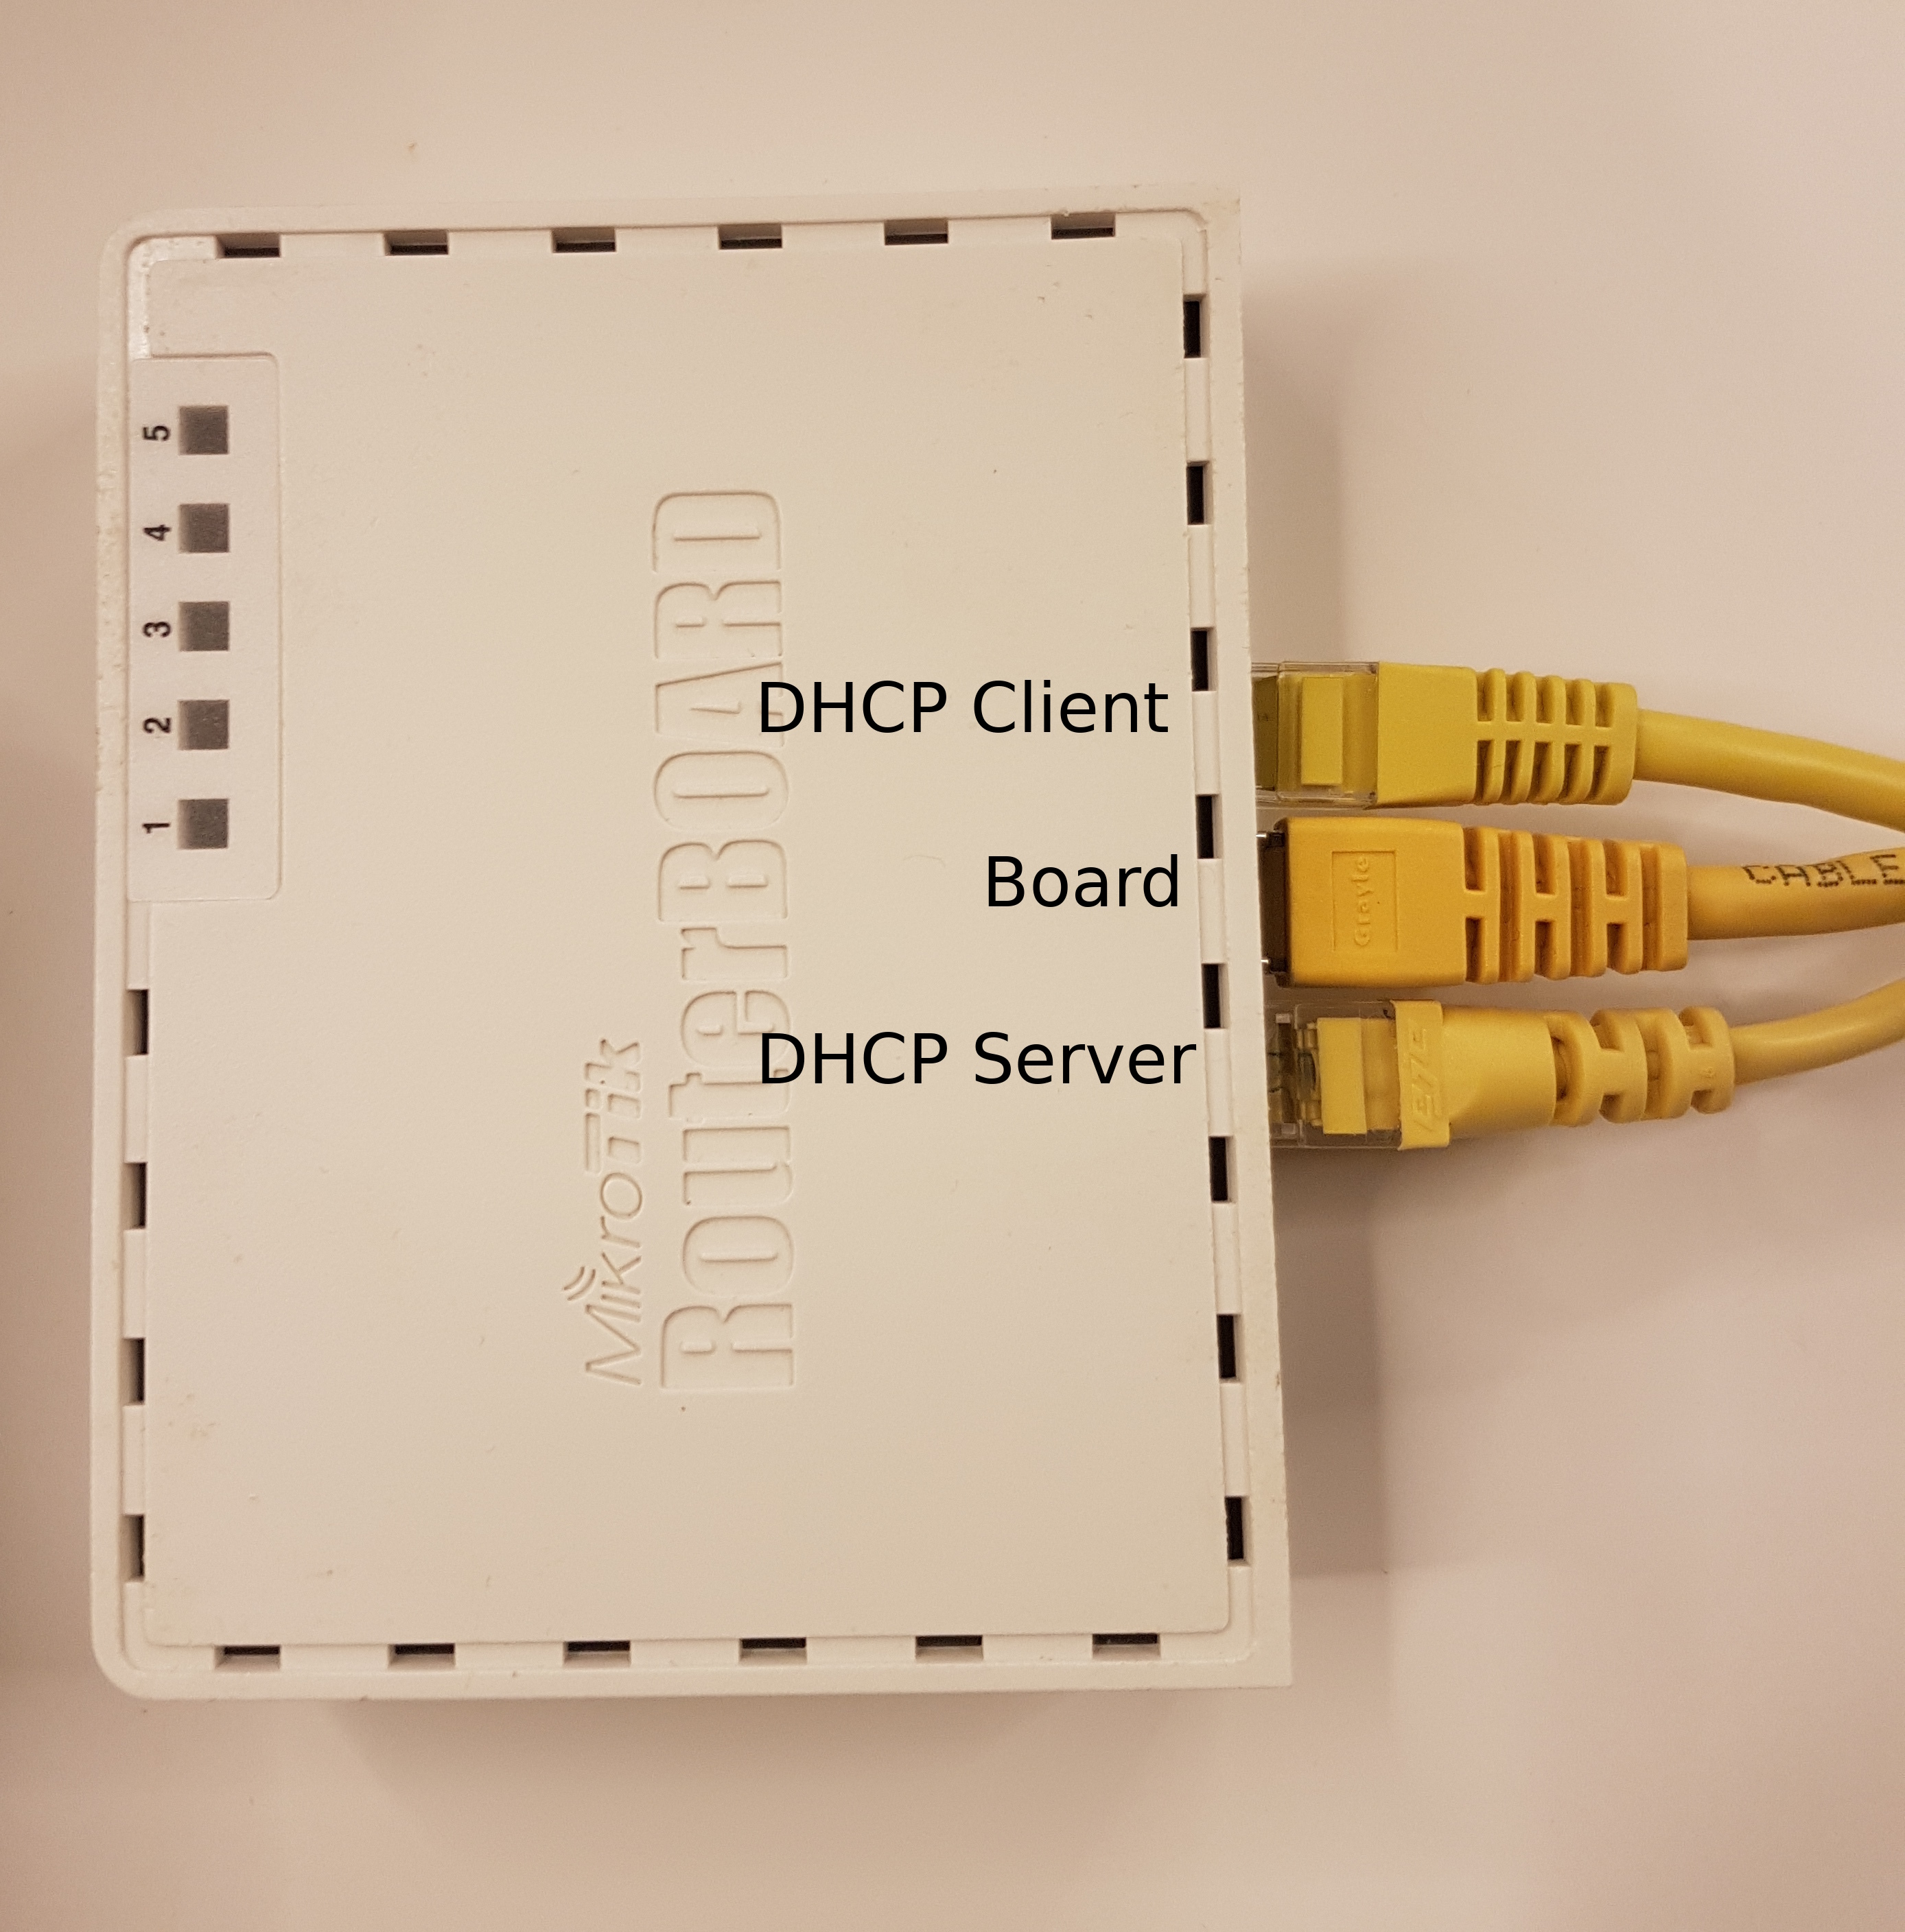
\includegraphics[scale=0.7]{images/router}
	\caption{Router wiring}
	\label{fig:router}
\end{figure}

Server and clients are supposed to belong to two different networks (otherwise a relay would not be necessary, as they could communicate ``directly''). The server must be connected to Port 1. The relay and the client(s) must be connected to ports from 2 to 5. A user can use these ports interchangeably. In Figure~\ref{fig:router}, relay and client are connected to Port 2 and 3, respectively. 

You should set you Ethernet interface to require an IP address assigned dynamically (in other words, you should not specify a static IP address).\\

The board (henceforth called \textit{relay}) displays a number of messages to let the client know what is going on. For instance, \textit{Send to client} means it is dispatching a packet (coming from the server) to you. General purpose messages, such as the previous one, are displayed on the first line of the LCD screen. Assigned IP addresses, on the other hand, are displayed on the second line. Seeing such an address means that you are about to receive it.

When started up, the LCD screen reads \textit{Waiting client} on the first line and the relay's IP address on the second. Such a configuration means you can connect your computer and wait for an address.

The right-most LED blinks to signal that the relay is up and running.